\documentclass{article}
\usepackage[utf8]{inputenc}
%\usepackage [danish]{babel} % Vi burde ikke have brug for den her
\usepackage[a4paper, hmargin={2.8cm, 2.8cm}, vmargin={2.5cm, 2.5cm}]{geometry}
\usepackage{eso-pic} % \AddToShipoutPicture
\usepackage{graphicx} % \includegraphics

% Så er der header
\usepackage{fancyhdr}
\setlength{\headheight}{15.2pt}
\pagestyle{fancy}
\rhead[\today]{\today}

\usepackage{wrapfig, blindtext}
\usepackage{array}
\usepackage{import}
\usepackage[hidelinks]{hyperref}
\usepackage{verbatim}
\usepackage{algorithm}
\usepackage{float}
\linespread{1.2}
\usepackage{pbox}
\usepackage{amsthm}
\usepackage{mathtools}
\usepackage{amsmath}
\usepackage{url}
\usepackage{listings}
\lstset{language=C++,
           basicstyle=\ttfamily,
           keywordstyle=\color{blue}\ttfamily,
           stringstyle=\color{red}\ttfamily,
           frame = single,
           commentstyle=\color{green}\ttfamily,
           breaklines=true,
           numbers=left
          }
\usepackage[toc,page]{appendix}
\usepackage{tikz}
\usetikzlibrary{arrows,automata,fit,positioning}
\usepackage{amsfonts}
\usepackage{standalone}
\newtheorem{theorem}{Teorem}
\newtheorem{lemma}{Lemma}
\newtheorem{korollar}{Korollar}
\newcolumntype{L}[1]{>{\raggedright\let\newline\\\arraybackslash\hspace{0pt}}m{#1}}
\newcolumntype{C}[1]{>{\centering\let\newline\\\arraybackslash\hspace{0pt}}m{#1}}
\newcolumntype{R}[1]{>{\raggedleft\let\newline\\\arraybackslash\hspace{0pt}}m{#1}}

\newcommand*\Let[2]{\State #1 $\gets$ #2}
\usepackage[noend]{algpseudocode}

\usepackage{algorithmicx}

\newtheorem{mydef}{Definition}
\newtheorem{myex}{Example}[section]
\usepackage{caption}
\DeclareMathOperator*{\argmin}{arg\,min}


\title{
  \vspace{3cm}
  \Huge{PMPH group project} \\
  \Large{Simon Nicolai Lefoli Maibom - xvm226} \\
  \Large{William Jack Lysgaard Sprent - pvw791}\\
  \Large{Edgar Antonio Sucar Escamilla - rbf271}
}

\usepackage{natbib}
\usepackage{graphicx}

\newcommand{\myfl}{\left\lfloor}
\newcommand{\myfr}{\right\rfloor}
\newcommand{\mycl}{\left\lceil}
\newcommand{\mycr}{\right\rceil}
\begin{document}

%% Change `ku-farve` to `nat-farve` to use SCIENCE's old colors or
%% `natbio-farve` to use SCIENCE's new colors and logo.
\AddToShipoutPicture*{\put(0,0){\includegraphics*[viewport=0 0 700 600]{natbio-farve}}}
\AddToShipoutPicture*{\put(0,602){\includegraphics*[viewport=0 600 700 1600]{natbio-farve}}}

%% Change `ku-en` to `nat-en` to use the `Faculty of Science` header
\AddToShipoutPicture*{\put(0,0){\includegraphics*{nat-en}}}

\clearpage\maketitle
\thispagestyle{empty}

\newpage
\tableofcontents
\newpage
\section{Loops and Structure of the program}
\subsection{Entry Point}
This loops acts as the entry-point for the program, encompassing close to all of the performed computation. It is not parallel in its
 current form. The variables \verb!strike! and \verb!globs! are both written to and read from in each iteration causing cross-iteration
 dependencies. However, they are both immeditely overwritten, \verb!globs! in the first three lines of \verb!value!, so the dependencies
 cannot be true dependencies and the loop is parallisable.
\begin{lstlisting}[caption=Outermost loop, label=outerloop]
REAL strike;
PrivGlobs    globs(numX, numY, numT);

for( unsigned i = 0; i < outer; ++ i ) {
      strike = 0.001*i;
      res[i] = value( globs, s0, strike, t,
                      alpha, nu,    beta,
                      numX,  numY,  numT );
}
\end{lstlisting}

\subsection{Second level}

\paragraph{setPayoff}
This 2-dimensional loop found in the \verb!setPayoff! function contains a trivially parallel inner-nest.
 However, the outer nest is not parallel due to a read-after-write
 dependency between the statements on line 3 and 5.
\begin{lstlisting}[caption=setPayoff() loop, label=payoffloop]
for(unsigned i=0;i<globs.myX.size();++i)
{
	REAL payoff = max(globs.myX[i]-strike, (REAL)0.0);
	for(unsigned j=0;j<globs.myY.size();++j)
		globs.myResult[i][j] = payoff;
}
\end{lstlisting}

\paragraph{Time}
This loop is inherently sequential. Each iteration uses reads and writes to arrays that are part \verb!globs! making
 each iteration dependant on the previous.
\begin{lstlisting}[caption=Timeline loop, label=timeloop]
for(int i = globs.myTimeline.size()-2;i>=0;--i)
    {
        updateParams(i,alpha,beta,nu,globs);
        rollback(i, globs);
    }
\end{lstlisting}

\subsection{Third level}
\label{sec:third}

\paragraph{updateParams}
This loop is trivially parallel in both loop nests as it does not write to any of the locations it reads from, and
 doesn't write to the same location twice.
\begin{lstlisting}[caption=Loop in updateParams(), label=updpar]
for(unsigned i=0;i<globs.myX.size();++i)
   for(unsigned j=0;j<globs.myY.size();++j) {
       globs.myVarX[i][j] = exp(2.0*(  beta*log(globs.myX[i])
                                     + globs.myY[j]
                                     - 0.5*nu*nu*globs.myTimeline[g])
                               );
       globs.myVarY[i][j] = exp(2.0*(  alpha*log(globs.myX[i])
                                     + globs.myY[j]
                                     - 0.5*nu*nu*globs.myTimeline[g])
                               );
   }
\end{lstlisting}

\subsubsection{Rollback}
\begin{lstlisting}[caption=Explicit x loop, label=exloop]
  for(i=0;i<numX;i++) {
        for(j=0;j<numY;j++) {
            u[j][i] = dtInv*globs.myResult[i][j];

            if(i > 0) {
              u[j][i] += 0.5*( 0.5*globs.myVarX[i][j]
                                  *globs.myDxx[i][0] )
                            * globs.myResult[i-1][j];
            }
            u[j][i]  +=  0.5*( 0.5*globs.myVarX[i][j]
                                  *globs.myDxx[i][1] )
                            * globs.myResult[i][j];
            if(i < numX-1) {
              u[j][i] += 0.5*( 0.5*globs.myVarX[i][j]
                                  *globs.myDxx[i][2] )
                            * globs.myResult[i+1][j];
            }
        }
    }
\end{lstlisting}
\begin{lstlisting}[caption=Explicit y loop, label=eyloop]
    for(j=0;j<numY;j++)
    {
        for(i=0;i<numX;i++) {
            v[i][j] = 0.0;

            if(j > 0) {
              v[i][j] +=  ( 0.5*globs.myVarY[i][j]
                               *globs.myDyy[j][0] )
                         *  globs.myResult[i][j-1];
            }
            v[i][j]  +=   ( 0.5*globs.myVarY[i][j]
                               *globs.myDyy[j][1] )
                         *  globs.myResult[i][j];
            if(j < numY-1) {
              v[i][j] +=  ( 0.5*globs.myVarY[i][j]
                               *globs.myDyy[j][2] )
                         *  globs.myResult[i][j+1];
            }
            u[j][i] += v[i][j];
        }
    }
\end{lstlisting}
\begin{lstlisting}[caption=Implicit x loop, label=impxloop]
for(j=0;j<numY;j++) {
    for(i=0;i<numX;i++) {
        a[i] =		 - 0.5*(0.5*globs.myVarX[i][j]*globs.myDxx[i][0]);
        b[i] = dtInv - 0.5*(0.5*globs.myVarX[i][j]*globs.myDxx[i][1]);
        c[i] =		 - 0.5*(0.5*globs.myVarX[i][j]*globs.myDxx[i][2]);
    }
    tridag(a,b,c,u[j],numX,u[j],yy);
}
\end{lstlisting}
\begin{lstlisting}[caption=Implicit y loop, label=impyloop]
for(i=0;i<numX;i++) {
     for(j=0;j<numY;j++) {
         a[j] =		 - 0.5*(0.5*globs.myVarY[i][j]*globs.myDyy[j][0]);
         b[j] = dtInv - 0.5*(0.5*globs.myVarY[i][j]*globs.myDyy[j][1]);
         c[j] =		 - 0.5*(0.5*globs.myVarY[i][j]*globs.myDyy[j][2]);
     }
      for(j=0;j<numY;j++)
         y[j] = dtInv*u[j][i] - 0.5*v[i][j];

     tridag(a,b,c,y,numY,globs.myResult[i],yy);
 }
\end{lstlisting}


\section{Transformations}

\subsection{Array Expansion}
\label{sec:arrayexp}

\subsection{Nest interchange and loop distribution}

\subsubsection{Structural}
\paragraph{Interchanging the outer loop inwards}
\subparagraph{Motivation:} In the original structure of the program, we have that a whole slew of loops
 (all of the loops in section \ref{sec:third}) are nested
 within the sequential time iterating loop (Listing \ref{timeloop}) which itself is positioned within
 the outer loop (Listing \ref{outerloop}). Meaning that we in general had 4-tiered loop nests of the following
 structure.
$$\mathrm{parallel} \to \mathrm{sequential} \to \mathrm{parallel} \to \mathrm{parallel}$$
We would prefer to have any sequential loops in the outer nests so that we can more effectively
 parallelise.
\subparagraph{Action:} Performed a nest interchange on the outer and time loops, moving the outer loop inwards.
\subparagraph{Result:} New structure where parallel loops are nested within the sequential loop.
$$\mathrm{sequential} \to \mathrm{parallel} \to \mathrm{parallel} \to \mathrm{parallel}$$
\subparagraph{Validity:} Moving a parallel loop inwards is always valid.

\paragraph{Distribution of Implicit x \& y loops}
\subparagraph{Motivation:} Currently the implicit x/y (Listing \ref{impxloop} \& \ref{impyloop}) consist of one or two loops along with a call
 to \verb!tridag!. We would prefer perfect loop nests.
\subparagraph{Action:} Distribute the secondmost inner nest across the innermost nests.
\subparagraph{Result:} Two/three (for x/y) perfect loop nests.
\subparagraph{Validity:} All used arrays are already array expanded as per section \ref{sec:arrayexp}.
\paragraph{Distributing the outer loop}
\subparagraph{Motivation:} Moving the outer loop inwards, leaves us with a big parallel loop nesting smaller double nested parallel loop
 (Figure \ref{fig:bintouter}.
 These inner loops all have different dimensions making it difficult to make a cohesive parallisation across them all. We would much
 prefer mutliple triple-tiered loops with perfect loop nests.\\
 \begin{figure}[h!]
   \centering
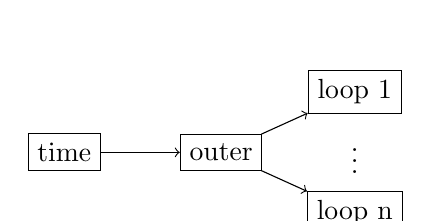
\begin{tikzpicture}[every node/.style={draw,rectangle}]
     \node (time) {time}; \node [right= of time] (outer) {outer};
     \node [right= of outer, draw = none] (dot) {$\vdots$}; \node
     [above= 0.1cm of dot] (1) {loop 1}; \node [below= 0.1cm of dot]
     (2) {loop n};

     \path [->] (time) edge (outer) [->] (outer) edge (1) edge (2);
   \end{tikzpicture}
   \caption{Loop nesting before interchange of outer}
   \label{fig:bintouter}
 \end{figure}
\subparagraph{Action:} Distribute the outer loop across its contained loops.
\subparagraph{Result:} All loops that had an outer-dimension are now perfect loop nests with the structure in Figure \ref{fig:aintouter}.
\begin{figure}[h!]
  \centering
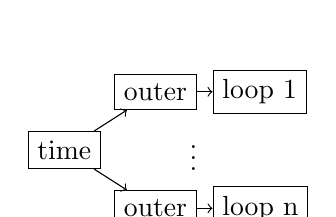
\begin{tikzpicture}[every node/.style={draw,rectangle}]
    \node (time) {time}; \node [right= of time, draw = none] (dot)
    {$\vdots$}; \node [above right= 0.1cm of dot] (1) {loop 1}; \node
    [below right= 0.1cm of dot] (2) {loop n}; \node [left= 0.2cm of 2]
    (outer2) {outer}; \node [left= 0.2cm of 1] (outer) {outer};

    \path [->] (time) edge (outer) edge (outer2) [->] (outer) edge (1)
    [->] (outer2) edge (2);
  \end{tikzpicture}
  \caption{Loop nesting after interchange of outer.}
  \label{fig:aintouter}
\end{figure}
\subparagraph{Validity:} This transformation is dependent on some of the already performed array expansions in section \ref{sec:arrayexp}.
 With these expansions, the transformation is valid. It does not change the order of execution within each iteration of the outer loop.
\subsubsection{Memory-motivated}

\paragraph{Loop interchanging for memory coalescence}
\subparagraph{Motivation:} Given that our working set of arrays are all stored in row-major order, we have that subsequent columns in the
 same row are stored subsequently in memory. To take advantage of spatial-locality and CUDA's memory banks we wish to iterate over columns
 in our innermost nests. This is not the case in loops such as the explicit y loop (Listing \ref{eyloop}).
\subparagraph{Action:} Interchange the two innermost loop nests where needed.
\subparagraph{Result:} Mostly improved memory access patterns. However, some variables - such as \verb!myVarX! in (Listing \ref{exloop}) -
 are now accessed uncoalesced.
\subparagraph{Validity:} Parallel loops can always be interchanged inwards.
\paragraph{Merging explicit \& implicit x/y}
\subparagraph{Motivation:} One of the loops resulting from each of the distribution of the implicit x/y loops are now on the form.
\begin{lstlisting}
  for i = 1..n
   for j = 1..m
    a[i][j] = ...
    b[i][j] = ...
    c[i][j] = ...
   endfor
  endfor
\end{lstlisting}
 Each statement of each iteration of these loops reference the same memory location as the earlier explicit x/y
 (Listings \ref{exloop} and \ref{eyloop}) such as to \verb!myVarX! - and now have the same nest structure. We wish make these loads just
 once for each iteration.
\subparagraph{Action:} Merge the explicit x and y loops with the corresponding implicit loop nests. Expand \verb!a!, \verb!b!, and \verb!c!
 to two arrays, i.e. \verb!ax! and \verb!ay!, as they can no longer be reused.
\subparagraph{Result:} Larger x and y loops.
\subparagraph{Validity:} The \verb!a!, \verb!b!, and \verb!c! arrays had been reused, so the validity of the transformation is dependent on
 the expansion of the two arrays.
\subsection{Transposition}



\section{Performance}

\subsection{Runtime}
\subparagraph{Setup:} All tests were performed on gpu2 of the GPU servers.

\subparagraph{Results:} 

30 run tests were run on each of the following program versions, with the total runtime (in microseconds) averaged:
\begin{itemize}
\item Original CPU implementation. Runtime average: 2450300.
\item Original CPU implementation with openmp on outer loop. Runtime average: 220008 .
\item Fully modified CPU implementation with openmp on parallel loops. Runtime average: 476647.
\item Final CUDA implementation. Runtime average: 390135.

Figure \ref{fig_res} shows a plot of the runtime in each test in the four configurations.
\end{itemize}
\begin{figure}[H]
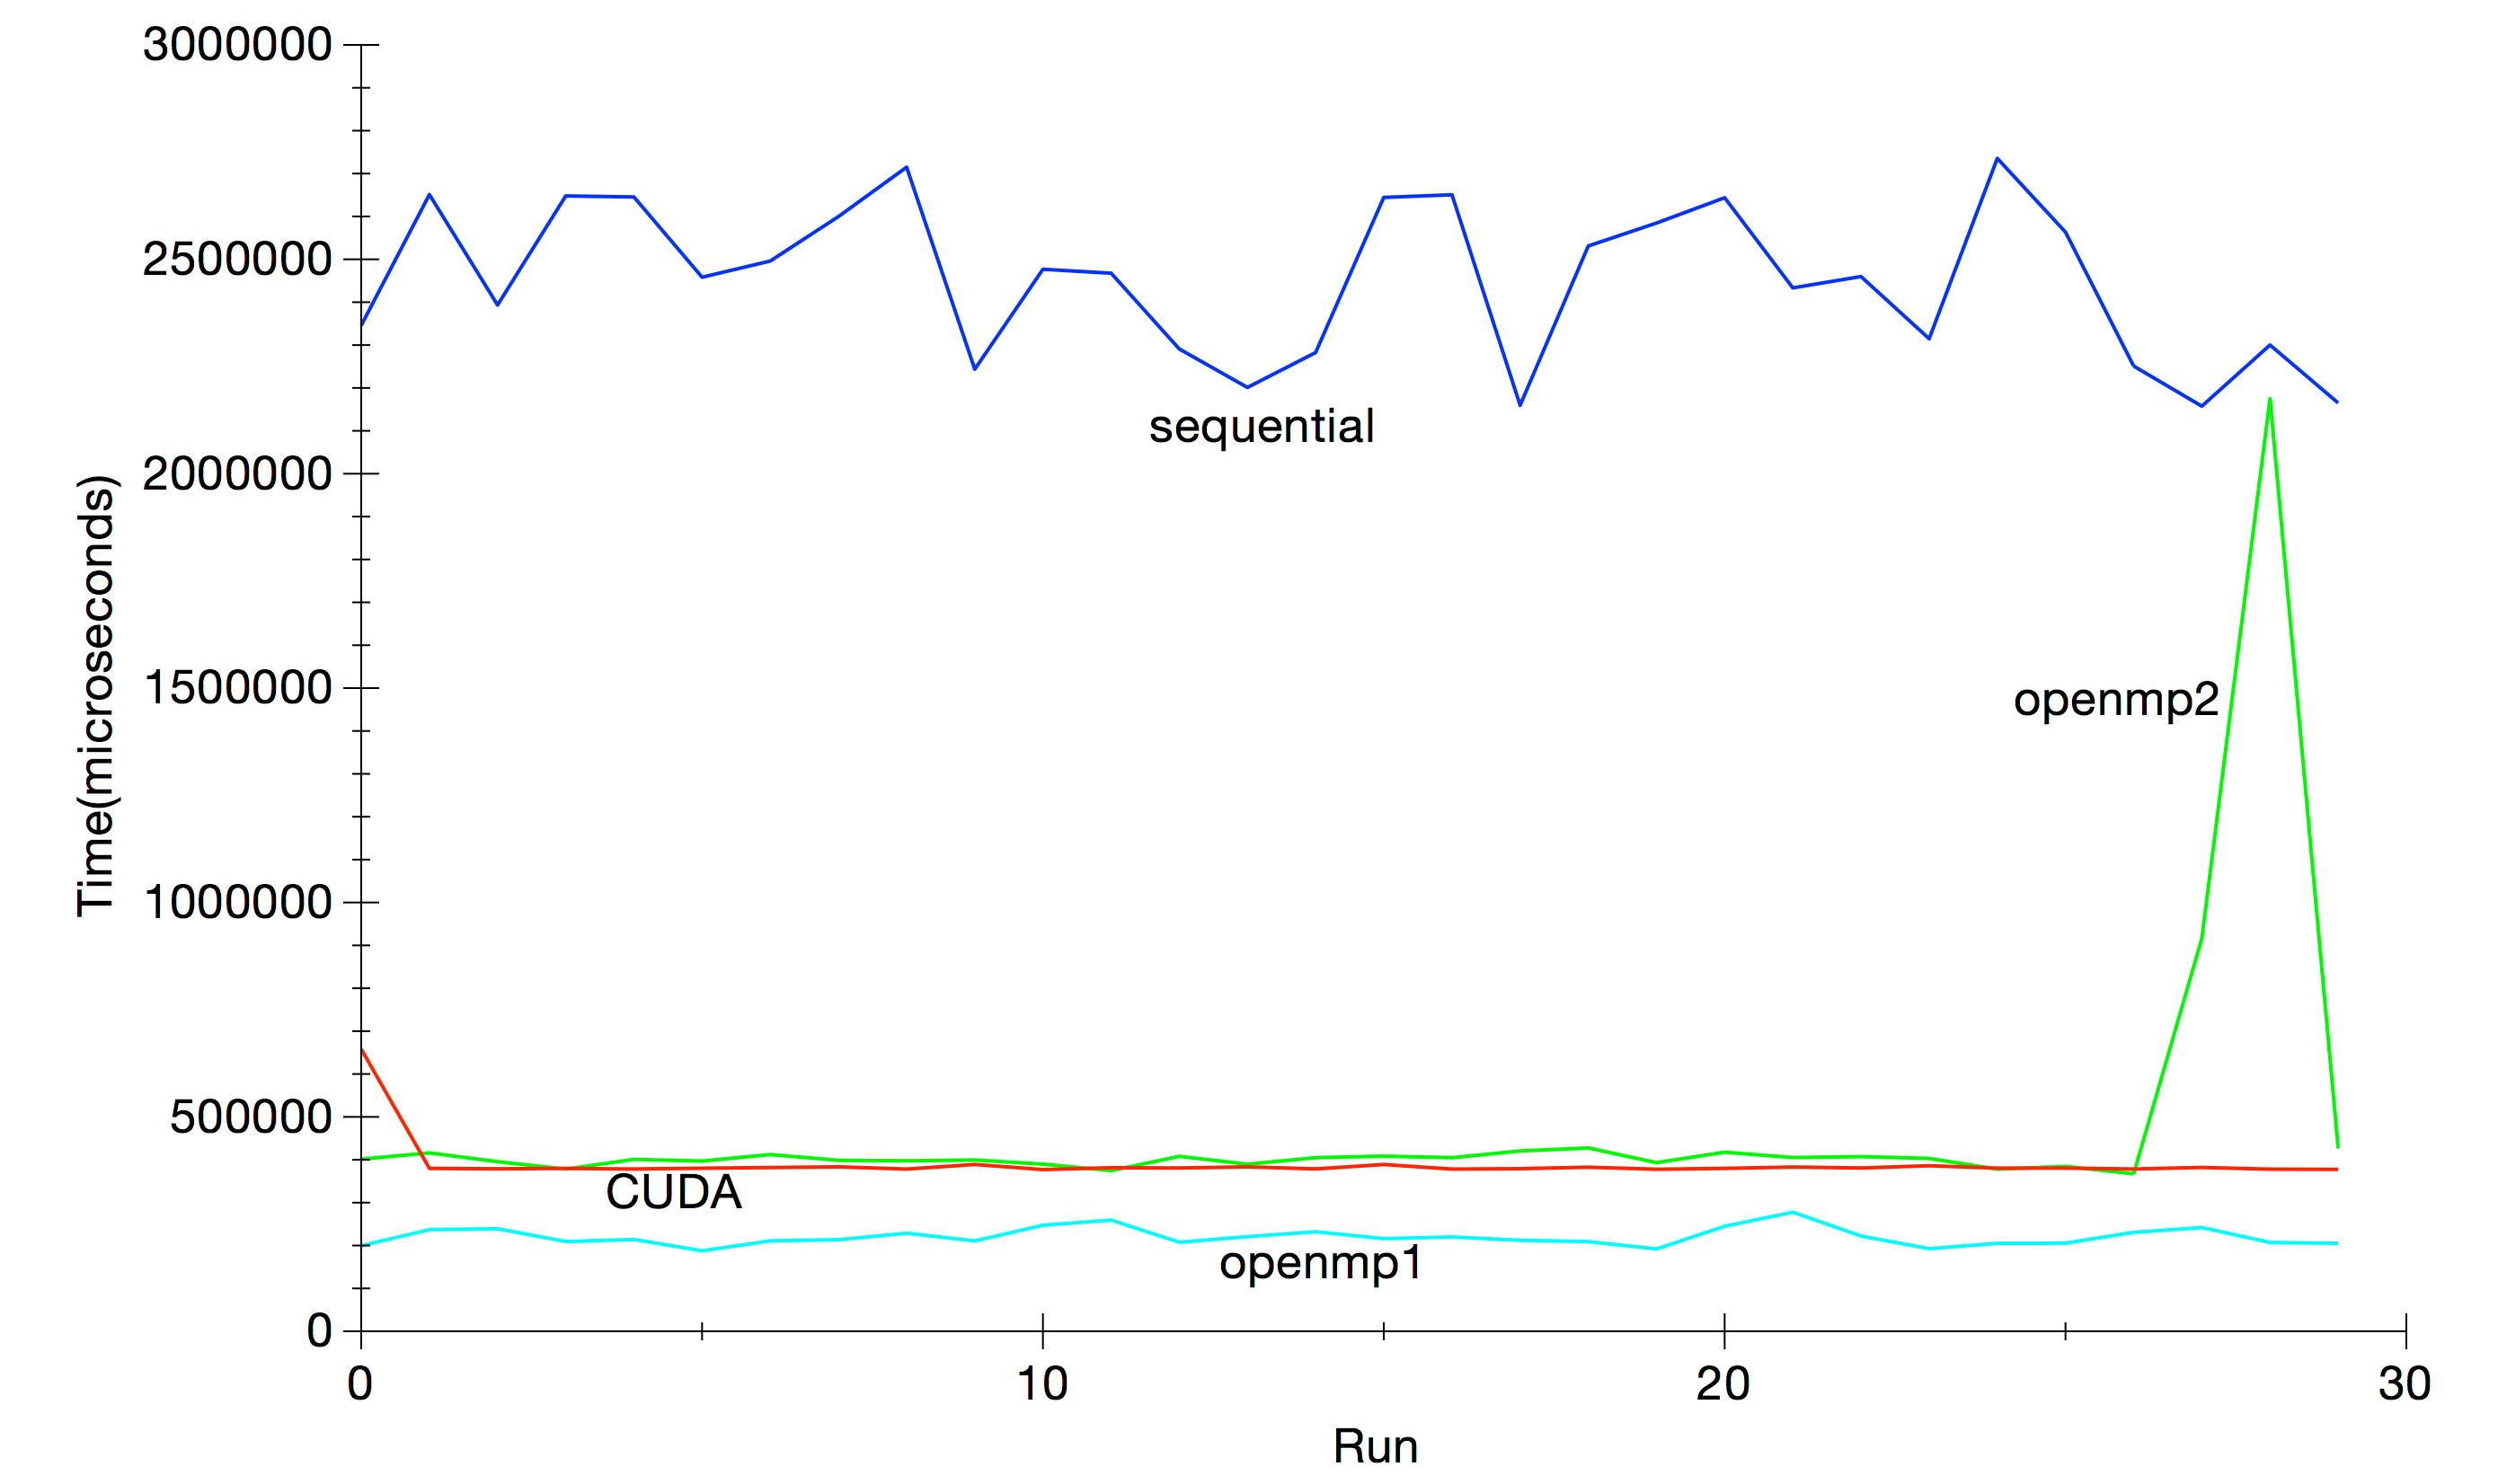
\includegraphics[width=150mm]{results_plot} 
\caption{Runtimes of the four program versions; sequential: original CPU implementation, openmp1: original CPU implementation with openmp on outer loop, openmp2: fully modified CPU implementation with openmp on parallel loops, and CUDA: final CUDA implementation.}
\label{fig_res}
\end{figure}


\subparagraph{Comments:} As expected the original CPU implementation has the highest runtime average by a recognizable margin. The parallelized versions of the code (with CUDA and openmp) have very similar runtimes, but the CUDA implementation has a lower runtime average due to an outlier in the openmp version runtimes. The orriginal CPU implementation with openmp on outer loop has the lowest runtime average, possible reasons are fewer overhead and memory faster access velocity of CPU over GPU. A lower runtime of the CUDA parallel version over the openmp one could be expected in a larger data set.

\subsection{Validation}
The results obtained in all tests were valid.

\section{Conclusion}
\subsection{Results}
We have successfully parallelised the program using CUDA. Our parallised program validates and manages to produce a significant speedup against
 the original implementation. However, it does not compete well with the CPU parallised version.
\subsection{Reflections}
Moving the a,b and c array calculations into the explicit x and y loops gave us no speedup. This resulted in doing unnecessary  array expansion instead. On the small dataset this is a neglectful decrease in speed however, but it could have a impact when using larger dimensions.

When parallising on GPU with a relatively small dataset such as we have, there is very little room for overhead and missing optimisations
 when competing
 with simple CPU parallisation. Our CUDA implementation, while faster than the original by a factor of 5, struggles to compete with the
 incredibly simple to implement OpenMP versions. This in stark difference compared to large bulk operations on large data sets,
 where CUDA can
 trivially achieve massive speedups due to its sheer degree of parallism.

\subsection{Further Improvement}
Currently we do not have kernels for the initialisation, we could move these calculations to the GPU and do it in parallel instead. It would save doing cudamemcpy calls for the dx, dy, dxx, dyy and myTimeline arrays, which would the overhead from cudamemcpy.
\end{document}
